\subsection{SHAP Evidence and Software-Module Suspect Ranking}

The explanation analysis was conducted on the 3602 anomalous test windows from the fixed chronological protocol. For each window, the TreeSHAP contributions of the predicted Stage 2 class were converted to absolute evidence and aggregated from statistical features to telemetry channels, PX4 topics, and subsystems. The aggregation preserved the total evidence mass: the maximum absolute conservation error across the hierarchy was $7.11 \times 10^{-15}$. This result verifies the numerical redistribution of the evidence, but it does not establish that the attributed channel or subsystem is the physical source of the anomaly.

The masking analysis tested whether the validation-derived SHAP ranking was more informative than an equal-size random feature selection. The top-$k$ SHAP features were ranked on validation anomaly windows and replaced in the test data by feature-wise medians calculated from the training windows. The Macro-F1 decrease for SHAP masking increased from 0.0409 at $k=10$ to 0.2683 at $k=100$. Across 20 random subsets nested within each of five model seeds, the paired SHAP-minus-random advantage was 0.0404 (95\% flight-log-bootstrap CI [0.0102, 0.0713]) at $k=10$ and 0.2646 [0.2052, 0.3300] at $k=100$. Replacing the selected feature block with values from sampled training rows produced drops of 0.0516 [0.0277, 0.0752] and 0.4955 [0.4604, 0.5283], respectively. The direction therefore persisted under both median and joint-donor perturbations, although donor replacement can still create cross-block combinations with unreplaced features. These results support prediction-relevant feature concentration, not causal influence or physical necessity.

At the telemetry-channel level, the original string-rule mapping and the document-derived mapping agreed on 76 of 87 channels. Under the document-derived reference, overall Consistency@1 was $0.2500 \pm 0.0056$, compared with the exact random baseline of 0.1707. Across $K \in \{1,3,5,10\}$, Consistency@K was $0.2500 \pm 0.0056$, $0.3494 \pm 0.0172$, $0.3410 \pm 0.0051$, and $0.2775 \pm 0.0028$, respectively. Class-level Consistency@1 was 0.0363 for External Position, 0.0349 for Global Position, 0.3779 for Altitude, and 0.8788 for Mechanical/Electrical; their respective random baselines were 0.0345, 0.1379, 0.1724, and 0.5402. Thus, External Position remained near random and Global Position fell below random after correcting semantically inappropriate axis-token assignments. The reduction from the original overall value of 0.3705 demonstrates material mapping sensitivity. Consistency@K is therefore not used as evidence of explanation correctness; it only describes agreement with a declared semantic reference.

For the architecture-aware layer, the static scan at commit \texttt{\seqsplit{82aa24adfca29321cfd1209e287eab6c2b16780e}} retained 180 topic-role-module edges covering 54 PX4 modules. The explicit-declaration audit comprised 244 occurrences across all 18 topics and produced role agreement and explicit-edge recall of 1.000 within its declared scope. Module evidence was then recomputed from only the 1,393 matching-commit anomalous test windows. Under producer-only propagation, the highest-ranked modules were \path{src/modules/ekf2} (SHAP share 0.2274), \path{src/modules/mavlink} (0.2068), \path{src/modules/sensors} (0.1036), \path{src/modules/position_estimator_inav} (0.0708), and \path{src/modules/load_mon} (0.0663). Figure~\ref{fig:shap_module_evidence}(d) now shows this version-coherent subset rather than the previous cross-version aggregate. Degree normalization materially changed the ordering: \path{position_estimator_inav} and \path{load_mon} ranked above \path{ekf2}, while the high-degree \path{mavlink} module fell to sixth. This sensitivity reinforces that the list is a propagation-dependent inspection aid, not a stable root-cause ranking.

The controlled-replay propagation ablation is reported in Table~\ref{tab:mapping_ablation}. Bidirectional propagation achieved Top-1/3/5 of 0.250/0.333/0.333 and MRR of 0.323, while producer-only and topic-only achieved higher Top-3 and Top-5 values of 0.500. The random-mapping control was lower, but the confidence intervals were wide and overlapping. With only 12 dependent mutation runs, the ablation does not identify a uniquely superior propagation rule.

\begin{table}[H]
\caption{Controlled-replay propagation ablation with 95\% two-way cluster-bootstrap confidence intervals. The bootstrap independently resamples the three source logs and four mutation types; the intervals remain low-resolution because both cluster counts are small.\label{tab:mapping_ablation}}
\centering
\scriptsize
\begin{tabularx}{\textwidth}{l c c c c}
\toprule
\textbf{Mode} & \textbf{Top-1 (95\% CI)} & \textbf{Top-3 (95\% CI)} & \textbf{Top-5 (95\% CI)} & \textbf{MRR (95\% CI)}\\
\midrule
Bidirectional & 0.250 [0.000, 0.583] & 0.333 [0.000, 0.750] & 0.333 [0.000, 0.750] & 0.323 [0.046, 0.679]\\
Producer-only & 0.250 [0.000, 0.583] & 0.500 [0.167, 0.833] & 0.500 [0.167, 0.833] & 0.414 [0.143, 0.690]\\
Consumer-only & 0.083 [0.000, 0.333] & 0.167 [0.000, 0.500] & 0.250 [0.000, 0.583] & 0.182 [0.035, 0.510]\\
Topic-only & 0.167 [0.000, 0.500] & 0.500 [0.167, 0.833] & 0.500 [0.167, 0.833] & 0.373 [0.147, 0.625]\\
Random mapping & 0.083 [0.000, 0.333] & 0.083 [0.000, 0.333] & 0.167 [0.000, 0.500] & 0.150 [0.031, 0.410]\\
\bottomrule
\end{tabularx}
\end{table}

Figure~\ref{fig:shap_module_evidence} summarizes the masking comparison, document-derived semantic-map agreement, class-specific Consistency@1, and the commit-matched module ranking. The complete internal analysis records are described in the Data Availability Statement.

\begin{figure}[H]
    \centering
    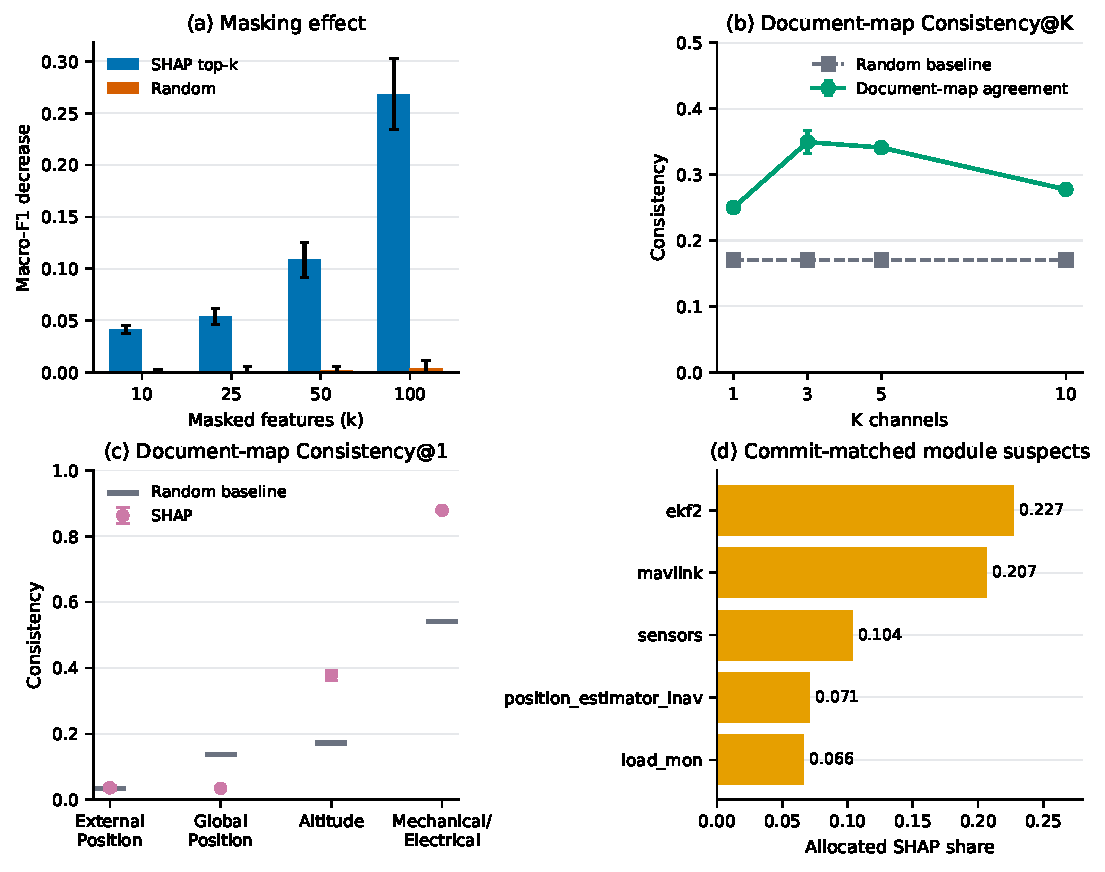
\includegraphics[width=\textwidth]{figures/figure_4_shap_evidence_module_ranking.pdf}
    \caption{SHAP evidence and architecture-aware module suspect ranking under the fixed chronological protocol. (a) Macro-F1 decrease after masking validation-ranked SHAP features or equal-size random subsets. (b) Overall agreement with the document-derived semantic mapping and exact random baselines. (c) Class-specific Consistency@1, showing near-random External Position and below-random Global Position agreement. (d) Producer-only module suspects recomputed from the 1,393 anomalous test windows whose firmware matches the selected PX4 commit. Error bars show seed standard deviations where reported.}
    \label{fig:shap_module_evidence}
\end{figure}
